\documentclass{article}
\usepackage{minted}
\usepackage{graphicx} % Required for inserting images
\newcommand{\pder}[2][]{\frac{\partial#1}{\partial#2}}
\newcommand{\spder}[2][]{\frac{\partial^2#1}{\partial#2^2}}

\title{Numerical Analysis of the Heat Equation}
\author{Alex Zhou}
\date{April 2019}

\begin{document}

\maketitle

\section{Introduction}

The heat equation is a well-known example of a parabolic equation and the analysis forms the basis of much research into other parabolic equations such as the Ricci flow or mean curvature flow in geometry.

The diffusion of heat in a bar of length \(L\) is described by the one-dimensional partial differential equation
\[ \pder[\theta]{t} = \kappa \spder[\theta]{x}, \quad 0 < x < L, \]
where \(\theta(x,t)\) is the temperature averaged over a cross-section \(A\) at distance \(x\) along the bar at time \(t\). Also, \(\kappa > 0\) is called the thermal diffusivity. 

We assume that there is negligible heat flux through the sides and the heat flux through a cross section at \(x\) is 
\[ -Ak \pder[\theta]{x}(\theta, t), \]
where \(A\) is the cross-sectional area and \(k\) is the thermal conductivity. Then the total heat between \(x \in [a, b]\) is 
\[ A\int_a^b \sigma\rho\theta(x,t)\,dx, \]
where \(\sigma\) is the specific heat and \(\rho\) is the density. The rate of change of total heat is then
\[ \frac{d}{dt}\left( A\int_a^b \sigma\rho\theta(x,t)\,dx \right) = A\sigma\rho\int_a^b \pder[\theta]{t}(x,t)\,dx. \]
This is equal to the heat flux out of \(x = b\) minus the heat flux into \(x = a\),
\[ -Ak\pder[\theta]{x}(a, t) + Ak\pder[\theta]{x}(b,t) = Ak\int_a^b \spder[\theta]{x}(x,t)\,dx, \]
which gives the heat equation with \(k = \kappa\sigma\rho\).

Suppose that at \(t \leq 0\), the bar has uniform temperature \(\theta_0\) and for \(t \geq 0\), the temperature at one end of the bar experiences an increase proportional to time, whilst the other end is maintained at a constant temperature or insulated. This gives rise to the initial condition
\[ \theta(x, 0) = \theta_0, \quad 0 < x < L, \]
and the boundary conditions
\[ \theta(0,t) = \theta_0 + \alpha t, \quad t > 0, \]
where \(\alpha > 0\) and 
\[ \mbox{either} \quad \theta(L, t) = \theta_0 \quad \mbox{or} \quad \pder[\theta]{t}(L,t) = 0, \quad t > 0. \]
\section{Analytic Solution for Semi-Infinite Domain}

Let us initially consider the case of a semi-infinite bar 
\[ \mbox{either} \quad \theta(x, t) \to \theta_0 \quad \mbox{or} \quad \pder[\theta]{t}(x,t) = 0, \quad \mbox{as} \quad x \to \infty, \quad t > 0. \]
Substitute
\[ \theta(x,t) = \theta_0 + \alpha tF(x,t), \]
where 
\[ F(x,t) = \frac{\theta - \theta_0}{\alpha t} ,\]
which is a dimensionless quantity, so is a function of dimensionless variables. Our problem has three variables, \(\kappa\), \(x\) and \(t\) and since \(\kappa\) has the same dimension as \(x^2 t^{-1}\), any dimensionless variable is a power of \(\xi = \frac{x}{\sqrt{\kappa t}}\). Therefore \(F(x,t) = F(\xi)\). 

Since \(\xi = 0\) when \(x = 0\) and \(\xi \to \infty\) as \(x \to \infty\), we have the new boundary conditions for \(F(\xi)\),
\[ F(0) = 1 \quad \mbox{and either} \quad F(\xi) \to 0  \quad \mbox{or} \quad F'(\xi) \to 0 \quad \mbox{as} \quad \xi \to \infty. \]
Note that the last boundary condition clear from
\[ \pder[\theta]{x} = \alpha t F'(\xi)\pder[\xi]{x} = \alpha \sqrt{\frac{t}{\kappa}}F'(\xi). \]
To compute the ODE for \(F(\xi)\), we differentiate again
\[ \spder[\theta]{x} = \alpha \sqrt{\frac{t}{\kappa}} F''(\xi) \pder[\xi]{x} = \frac{\alpha}{\kappa}F''(\xi), \]
and then compute the time derivative
\[ \pder[\theta]{t} = \alpha F(\xi) + \alpha t F'(\xi)\pder[\xi]{t} = \alpha F(\xi) - \frac{\alpha \xi}{2}F'(\xi). \]
Re-substituting into the heat equation and dividing by \(\alpha\) yields
\[ F''(\xi) + \frac{ \xi}{2}F'(\xi) - F(\xi) = 0. \]
The solution of the ODE requires the use of error functions. We can verify the following is a solution
\[ F(\xi) = \left(1 + \frac{\xi^2}{2}\right)\mathop{\mathrm{erfc}}\left(\frac{\xi}{2}\right) - \frac{\xi}{\sqrt{\pi}}\exp\left(-\frac{\xi^2}{4}\right), \]
where
\[ \mathop{\mathrm{erfc}}(s) = \frac{2}{\sqrt{\pi}}\int_s^\infty \exp(-u^2)\,du \]
solves the ODE. Indeed, differentiating the function gives us
\begin{eqnarray*}
    F'(\xi) & = & \xi \mathop{\mathrm{erfc}}\left(\frac{\xi}{2}\right) +  \left(1 + \frac{\xi^2}{2}\right)\left( -\frac{1}{\sqrt{\pi}}\exp\left(-\frac{\xi^2}{4}\right) \right) \\
            & & -\frac{1}{\sqrt{\pi}}\exp\left(-\frac{\xi^2}{4}\right) + \frac{\xi}{\sqrt{\pi}}\frac{\xi}{2}\exp\left(-\frac{\xi^2}{4}\right) \\
            & = & \xi \mathop{\mathrm{erfc}}\left(\frac{\xi}{2}\right) - \frac{2}{\sqrt{\pi}}\exp\left(-\frac{\xi^2}{4}\right),
\end{eqnarray*}
and differentiating again
\begin{eqnarray*}
    F''(\xi) & = & \mathop{\mathrm{erfc}}\left(\frac{\xi}{2}\right) + \xi\left(-\frac{1}{\sqrt{\pi}}\exp\left(-\frac{\xi^2}{4}\right) \right) - \frac{2}{\sqrt{\pi}}\left(-\frac{\xi}{2}\right)\exp\left(-\frac{\xi^2}{4}\right) \\
             & = & \mathop{\mathrm{erfc}}\left(\frac{\xi}{2}\right).
\end{eqnarray*}
Then substituting into the ODE
\begin{eqnarray*}
    F''(\xi) + \frac{\xi}{2}F'(\xi) - F(\xi) & = & 
    \mathop{\mathrm{erfc}}\left(\frac{\xi}{2}\right)
    + \frac{\xi^2}{2} \mathop{\mathrm{erfc}}\left(\frac{\xi}{2}\right) - \frac{\xi}{\sqrt{\pi}}\exp\left(-\frac{\xi^2}{4}\right) \\
    & & - \left(1 + \frac{\xi^2}{2}\right)\mathop{\mathrm{erfc}}\left(\frac{\xi}{2}\right) + \frac{\xi}{\sqrt{\pi}}\exp\left(\frac{\xi^2}{4}\right) = 0,
\end{eqnarray*} 
as required. Checking the boundary conditions, \(F(0) = 1\) comes from a computation of the standard Gaussian integral (using the polar coordinates trick), and as \(\xi \to \infty\), both terms tends to \(0\) by L'Hopital's rule, where the error function and the negative exponential both decay faster than any polynomial grows. The same also holds for \(F'(\xi)\) as \(\xi \to \infty\).

To check uniqueness, consider that our ODE is also satisfied by the solution \((\frac{\xi^2}{2} + 1)\) which i linearly independent from our first solution either by checking the Wronskian or noting the the first solution decays to \(0\) whilst the second diverges to \(\infty\) as \(\xi \to \infty\). By the superposition principle, the general solution is the linear combination of these two solutions, where the coefficient on the second solution is \(0\) by the second boundary condition.

\section{Finite Domain, Fixed Temperature End}
We now return to the case of a finite bar and define the non-dimensional variables \(X\), \(T\) and \(U\) by
\[ x = LX, \quad t = L^2\kappa^{-1}T, \quad \theta(x, t) = \theta_0 + \alpha L^2 \kappa^{-1} U(X, T). \]
The heat equation now transforms into
\[ \pder[U]{T} = \spder[U]{X}, \quad T > 0, \quad 0 < X < 1,  \]
with initial condition
\[ U(X, 0) = 0, \quad 0 < X < 1 \]
and boundary conditions
\[ U(0, T) = T \quad \mbox{and} \quad U(1, T) = 0. \]
To find an analytic solution, we first subtract the simplest function that satisfies the boundary conditions \(U(X, T) = T(1 - X) + V(X, T) \), where \(V\) satisfies
\[ 1-X + \pder[V]{T} = \spder[V]{X}, \quad V(0, T) = 0, \quad V(1, T) = 0, \]
and noting that there is a particular solution with \(V\) independent of \(T\), we subtract that away
\[ V(X, T) = -\frac{1}{3}X + \frac{1}{2}X^2 - \frac{1}{6}X^3 + W(X, T), \]
to obtain the homogeneous problem
\[ \pder[W]{T} = \spder[W]{X}, \quad W(0, T) = 0, \quad W(1, T) = 0, \]
which has separable solutions for \(W\). Consider \(W(X, T) = A(X)B(T) \). By plugging into the ODE, we get
\[ \frac{B'(T)}{B(T)} = \frac{A''(X)}{A(X)} = -\lambda \]
for some constant \(\lambda\). By considering the characteristic equation for the ODE \(A'' + \lambda A = 0\), we see that we must have \(\lambda > 0\) for a non-trivial solution. Therefore
\[ A(X) = C'_1\cos(\sqrt{\lambda}X) + C'_2\sin(\sqrt{\lambda}X). \]
Using the boundary conditions, \(A(0) = 0\) implies \(C'_1 = 0\) whilst \(A(1) = 0\) implies \(\sin\sqrt\lambda = 0\), which means \(\lambda = (n\pi)^2\) for positive integer \(n\). Consequently, \(B\) must satisfy \(B' + (n\pi)^2B = 0\) which has solution
\[ B(T) = C_n\exp(-(n\pi)^2T). \]
Combining both of these functions gives us a general solution for \(W\),
\[ W(X, T) = \sum_{n=1}^\infty c_n\sin(n\pi X) \exp(-(n\pi)^2T). \]
To account for the initial condition \(U(X, 0) = 0\), we choose \(c_n\) such that
\[ \sum_{n=1}^\infty c_n \sin(n \pi X) = W(X, 0) = \frac{1}{3}X - \frac{1}{2}X^2 + \frac{1}{6}X^3 \]
By the orthogonality of sines, 
\[ 2\int_0^1 \sin(m\pi X)\sin(n\pi X) \,dX = \delta_{m,n}, \]
we can multiple both sides of by \(\sin(m\pi X)\) and integrate over \([0,1]\). Assuming we can swap the sum and the integral,
\[ \sum_{n=1}^\infty \int_0^1 c_n\sin(m\pi X)\sin(n\pi X) \,dX = \int_0^1 \sin(m\pi X)\left(\frac{1}{3}X - \frac{1}{2}X^2 + \frac{1}{6}X^3\right)  \,dX  \]
and the left hand side is exactly \(\frac{1}{2}c_m\) by orthogonality. In turns out by heavy use of integration by parts that
\[ c_n = \frac{2}{(n\pi)^3}. \]
As \(T \to \infty\), the lowest mode dominates because of the \(\exp(-(n\pi)^2 T)\) term. Thus to examine the limiting behaviour, it suffices to consider the first sine Fourier term. Then by the above formulae
\[ W(X, T) \sim \frac{2}{\pi^3} \sin(\pi X) \exp(-\pi^2 T) \quad \mbox{as} \quad T \to \infty. \]

\section{Finite Domain, Insulated End}

Using a similar technique, consider the transformed heat equation as before
\[ \pder[U]{T} = \spder[U]{X}, \quad T > 0, \quad 0 < X < 1,  \]
with initial condition
\[ U(X, 0) = 0, \quad 0 < X < 1, \]
but now with the boundary condition
\[ U(0, T) = T \quad \mbox{and} \quad \pder[U]{T}(1, T) = 0, \quad T > 0. \]
Similarly, we subtract the simplest function that satisfies the boundary conditions
\(U(X, T) = T + V(X, T), \)
which means
\[ 1 + \pder[V]{T} = \spder[V]{X}, \quad V(0,T) = 0, \quad \pder[V]{X}(1, T) = 0. \]
Subtracting off the particular solution which is independent of \(T\)
\[ V(X, T) = \frac{1}{2}X^2 - X + W(X, T), \]
yielding the homogeneous problem
\[ \pder[W]{T} = \spder[W]{X},\quad W(0,T) = 0, \quad \pder[W]{T}(1, T) = 0. \]
Separation of variables \(W(X, T) = A(X)B(T)\) with \(A(0) = 0\) gives the same general solution
\[ A(X) = C'_2\sin(\sqrt{\lambda}X), \]
but now \(A'(1) = 0\) means \(\cos(\sqrt{\lambda}) = 0\), therefore \(\lambda = ((n-\frac{1}{2})\pi)^2\) for positive integer \(n\). Once again, solving the ODE for \(B\) yields the general solution
\[ W(X, T) = \sum_{n=1}^\infty c_n \sin\left((n - 1/2)\pi X\right)\exp\left(-\left((n - 1/2)\pi\right)^2T\right). \]
Finally, considering the initial condition \(U(X, 0) = 0\) or \(W(X, T) = -\frac{1}{2}X^2 +X\), we compute the Fourier coefficients using orthogonality,
\[ c_n = \frac{2}{((n-1/2)\pi)^3}, \]
where we also have
\[ W(X, T) \sim \frac{2}{((1/2)\pi)^3} \sin((1/2)\pi X) \exp(-((1/2)\pi)^2 T) \quad \mbox{as} \quad T \to \infty, \]
since the first term dominates.

\section{Visualisations}
We plot the non-dimensional profiles \(U(X, T)\) against \(X\) for times
\[ T = 0.03125, 0.125, 0.25, 0.375, 0.75, 1.5, \]
for the fixed end, insulated end and semi-infinite end \((\theta(X, T) = TF(X, T))\) cases. To analyse how many terms in the power series we should take, let \(N\) be a positive integer. Then the trailing sums after \(N\) for the solution \(W(X, T)\) of the fixed temperature end problem satisfy
\begin{eqnarray*} 
    \left|\sum_{n > N} \sin(n\pi X)\exp(-(n\pi)^2T)\right| & \leq & \sum_{n > N} \left|  \sin(n\pi X)\exp(-(n\pi)^2T)\right| \\
    & \leq & \sum_{n > N} \exp(-(n\pi)^2T) \\
    & \leq & \sum_{n > N} \exp(-n\pi^2T) \\
    & \leq &  \frac{\exp(-N\pi^2T)}{1 - \exp(-\pi^2T)}, \\
\end{eqnarray*}
which is less than \(10^{-6}\) for \(T \geq 0.03125\) if we choose \(N = 20\). We first tabulate \(U(X, T)\) for all three solutions at \(T = 0.25\) and \(X = 0.125n\) for \(n = 0, \dots, 8\).
\begin{verbatim}[Output]
    x       Fixed       Insulated   Semi-Infinite
    0.0     0.25        0.25        0.25
    0.125   0.186664    0.18718     0.186922
    0.25    0.136681    0.137884    0.137282
    0.375   0.097828    0.100094    0.098961
    0.5     0.06797     0.071959    0.069965
    0.625   0.045093    0.051865    0.048479
    0.75    0.027305    0.038493    0.032899
    0.875   0.012835    0.030868    0.021852
    1.0     0.0         0.028394    0.014198
\end{verbatim}
Notice that the boundary condition \(U(0,T) = T\) is satisfied for all three cases. The initial condition \(U(X, 0) = 0\) gives us the behaviour for a short time. For a fixed small time, the heat in the bar has a sharp drop initially as \(X\) increases.

\begin{figure}
    \centering
    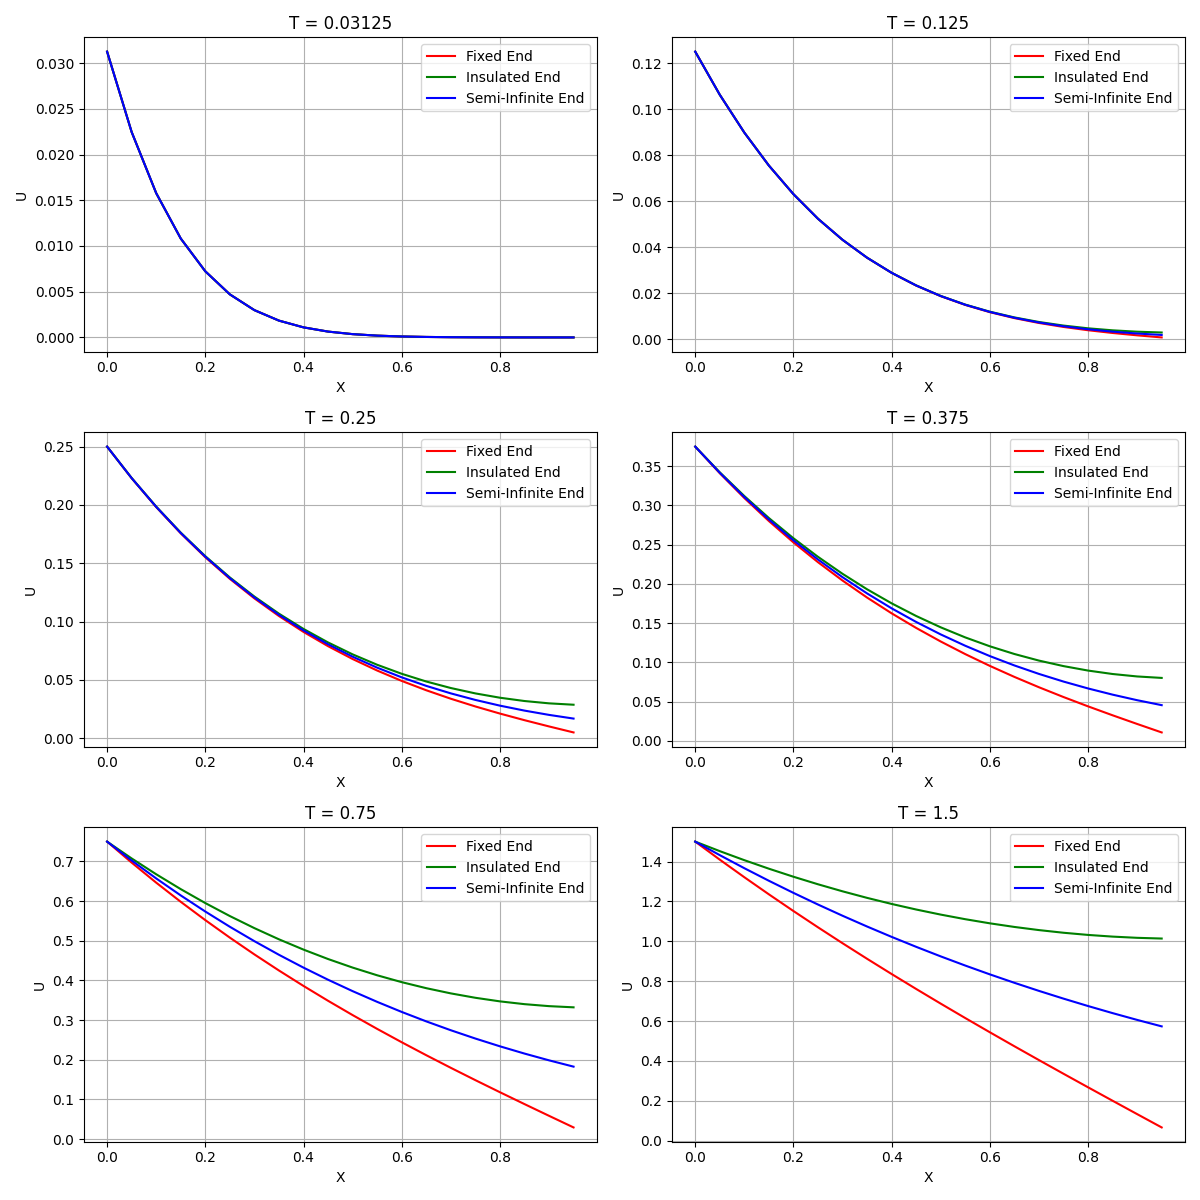
\includegraphics[width=1.0\linewidth]{images/heat_equation_all_cases.png}
    \caption{Plots of solutions to the heat equation for various times \(T\) with initial condition \(U(0,T) = T\).}
\end{figure}

Long term behaviour is governed by the second boundary condition at \(X = 1\) or at infinity. The constant temperature end solution converges to the steady state solution \(1-X\) whilst the insulated end solution converges to a constant solution \(1\). This is in part due to the exponential terms in the power series rapidly converging to \(0\). 

\begin{figure}
    \centering
    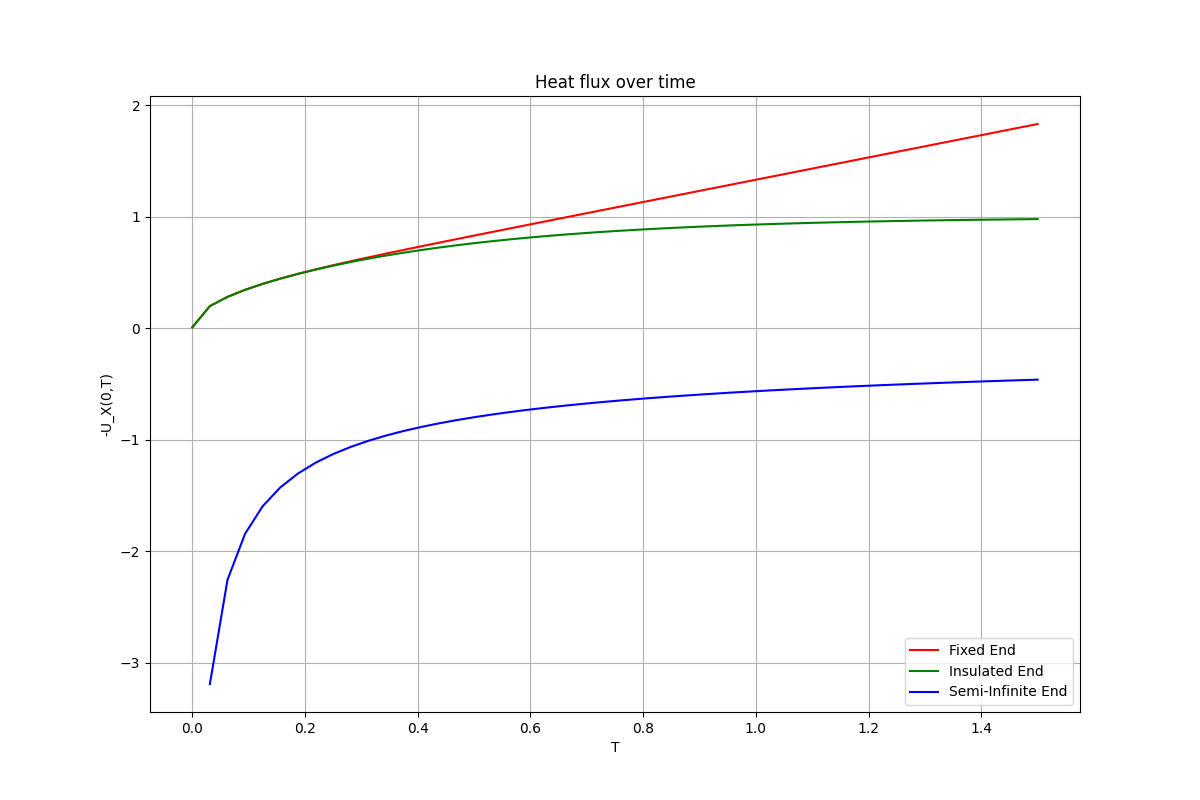
\includegraphics[width=1.0\linewidth]{images/flux.png}
    \caption{Heat flux \(-U(X,T)\) at \(X = 0\)}
\end{figure}

The semi-infinite solution shares properties of the other two solutions at infinity since both \(U(X,T)\) and \(\pder[U]{X}(X,T)\) tend to \(0\) as \(X \to \infty\). As \(T\) increases, the heat along the bar shifts upwards and the heat at a single point \(X\) tends to \(1\) as \(T \to \infty\).

The heat flux at \(X = 0\) increases for all three cases, which shows the sharp drop of the solutions upon a small increase in \(X\). This physically manifest itself as a very high temperature at the starting end of the bar which is adjacent to zero temperature. For the fixed temperature end, we would expect a linear decrease in temperature across the rod, whilst for the insulated end, since there is no flux out of the system, we expect the temperature eventually evolve into a constant temperature. The infinite end case has flux inversely proportional to \(\sqrt{T}\) which lies between the linear and constant cases.

\begin{minted}[autogobble, linenos]{python}
    pi = np.pi
    def u_1(x, t):
        boundary = t * (1 - x)
        particular = -x/3 + x**2/2 - x**3/6
        general = sum([(2/(n*pi)**3) * np.sin(n*pi*x) * np.exp(-(n*pi)**2 * t) for n in range(1, 20)])
        return boundary + particular + general
    def u_2(x, t):
        boundary = t
        particular = -x + x**2/2
        general = sum([(2/((n-0.5)*pi)**3) * np.sin((n-0.5)*pi*x) * np.exp(-((n-0.5)*pi)**2 * t) for n in range(1, 20)])
        return boundary + particular + general
    def u_3(x, t):
        f = lambda xi: (1 + xi**2/2) * math.erfc(xi/2) - xi * np.exp(-xi**2/4) / np.sqrt(pi)
        return t * f(x / np.sqrt(t))

    ux_1 = lambda t: - t - 1/3 + sum([ (2/(n*pi)**2) * (np.exp(-(n*pi)**2 * t)) for n in range(1, 25)])
    ux_2 = lambda t: - 1 + sum([ (2/((n - 0.5)*pi)**2) * (np.exp(-((n-0.5)*pi)**2 * t))  for n in range(1, 25)])
    ux_3 = lambda t: np.sqrt(1) / np.sqrt(pi * t)
\end{minted}

\section{Numerical Solution using Finite Time-Centred Space}

We now move on to solve the heat equation for \(U(X,T)\) numerically. Divide the domain \([0,1]\) into \(N\) intervals of length \(\Delta X = \frac{1}{N}\) and let \(\pder[U]{T}\) be approximated by a forward difference in time
\[ \pder[U]{T}(X,T) = \frac{U(X, T + \Delta T) - U(X,T)}{\Delta T} + O(\Delta T), \]
and \(\spder[U]{X}\) by a centred difference in space at the current time
\[ \spder[U]{X}(X, T) = \frac{U(X + \Delta X, T) - 2U(X, T) + U(X - \Delta X, T)}{(\Delta X)^2} + O((\Delta X)^2), \]
which gives the forward time centred space (FTCS) numerical scheme
\[ U_n^{m+1} = U_n^m + C(U_{n+1}^m -2U_n^m + U_{n-1}^m), \]
where \(U_n^m\) is an approximation to \(U(n\Delta X, m\Delta T)\) and \(C = \Delta T / (\Delta X)^2\) is the Courant number. To account for the initial condition, we simply set \(U_n^0 = 0\) for all \(n\). For the boundary condition, we update the boundary each time. This is not strictly necessary for the constant temperature end where we set
\[ U_N^{m+1} = 0,\]
but we want to keep the code consistent and 'safe'. Indeed, for the insulated end, consider the symmetric central difference at \(X \in (1-\varepsilon, 1+\varepsilon)\) by extending the solution on this domain
\[ \pder[U]{X}(1, T) = \frac{U(1+\Delta X, T) - U(1-\Delta X, T)}{2\Delta X} + O(\Delta X) = 0. \]
Taking \(\Delta X \to 0\), 
\[ U(1+\Delta X, T) = U(1-\Delta X, T), \]
which translates to 
\[ U_N^{m+1} = U_{N-1}^{m+1} \]
applied after every space step.

The following Python program implements this scheme for the constant temperature end and the insulated end:

\begin{minted}[autogobble, linenos]{python}
    def ftcs_scheme(N, C, boundary_type):
        Dx = 1 / N
        Dt = C / N ** 2
        n_rows =  int(1 / Dx) + 1
        m_cols = int(1 / Dt) + 1
        print(Dt)
        
        U = np.zeros((n_rows, m_cols)) # Contains initial condition
        U[0, :] = np.arange(m_cols) * Dt # First boundary
        
        for m in range(m_cols - 1):
            for n in range(1, n_rows - 1):
                U[n, m+1] = U[n, m] + C * (U[n+1, m] - 2*U[n, m] + U[n-1, m])
            if boundary_type == 1:
                U[-1, m+1] = 0 # Fixed end
            elif boundary_type == 2:
                U[-1, m+1] = U[-2, m+1] # Insulated end
        print(Dx, Dt)
        return U
\end{minted}

To see this clearer, we shall tabulate and/or plot some graphs for various choices of \(N = 4, 8, 16, 32\), \(C = \frac{2}{3}, \frac{1}{2}, \frac{1}{3}, \frac{1}{6}, \frac{1}{12}\) and \(T = 0.125, 0.25, 0.375\). 

We first tabulate the analytic and numerical solutions for \(N = 4\) and \(C = \frac{1}{2}\) at times \(T = 0.125, 0.25, 0.375\). From now on, let us only focus on the constant temperature end boundary condition.

\begin{table}[ht!]
    \centering
    \begin{tabular}{|c|c|c|c|}
        \hline
        X & Numeric & Analytic & Error \\
        \hline\hline
        0.0 & 0.125 & 0.125 & 0.0 \\
        0.25 & 0.050781 & 0.052403 & -0.001622 \\
        0.5 & 0.015625 & 0.018784 & -0.003159 \\
        0.75 & 0.003906 & 0.005412 & -0.001506 \\
        1.0 & 0.0 & 0.0 & 0.0 \\
        \hline 
    \end{tabular}
    \caption{\(T = 0.125\)}
    \bigskip\bigskip
    
    \begin{tabular}{|c|c|c|c|}
        \hline
        X & Numeric & Analytic & Error \\
        \hline\hline
        0.0 & 0.25 & 0.25 & 0.0 \\
        0.25 & 0.135742 & 0.136681 & -0.000939 \\
        0.5 & 0.066406 & 0.06797 & -0.001564 \\
        0.75 & 0.026367 & 0.027305 & -0.000938 \\
        1.0 & 0.0 & 0.0 & -0.0 \\
        \hline
    \end{tabular}
    \caption{\(T = 0.25\)}
    \bigskip\bigskip

    \begin{tabular}{|c|c|c|c|}
        \hline
        X & Numeric & Analytic & Error \\
        \hline\hline
        0.0 & 0.375 & 0.375 & 0.0 \\
        0.25 & 0.227295 & 0.227689 & -0.000394 \\
        0.5 & 0.125977 & 0.126593 & -0.000616 \\
        0.75 & 0.05542 & 0.055814 & -0.000394 \\
        1.0 & 0.0 & 0.0 & -0.0 \\
        \hline
    \end{tabular}
    \caption{\(T = 0.375\)}
\end{table}

From the table, we notice that the error increases as \(T\) increases but still remains small in magnitude. This is confirmed in the following plots which seem to indicate stability for \(C = \frac{1}{12}\) at time \(T = 0.375\), but in contrast, for \(C = \frac{2}{3}\), we see large oscillations at  time \(T = 0.375\) that deviate heavily from the analytic solution. 

\begin{figure}
    \centering
    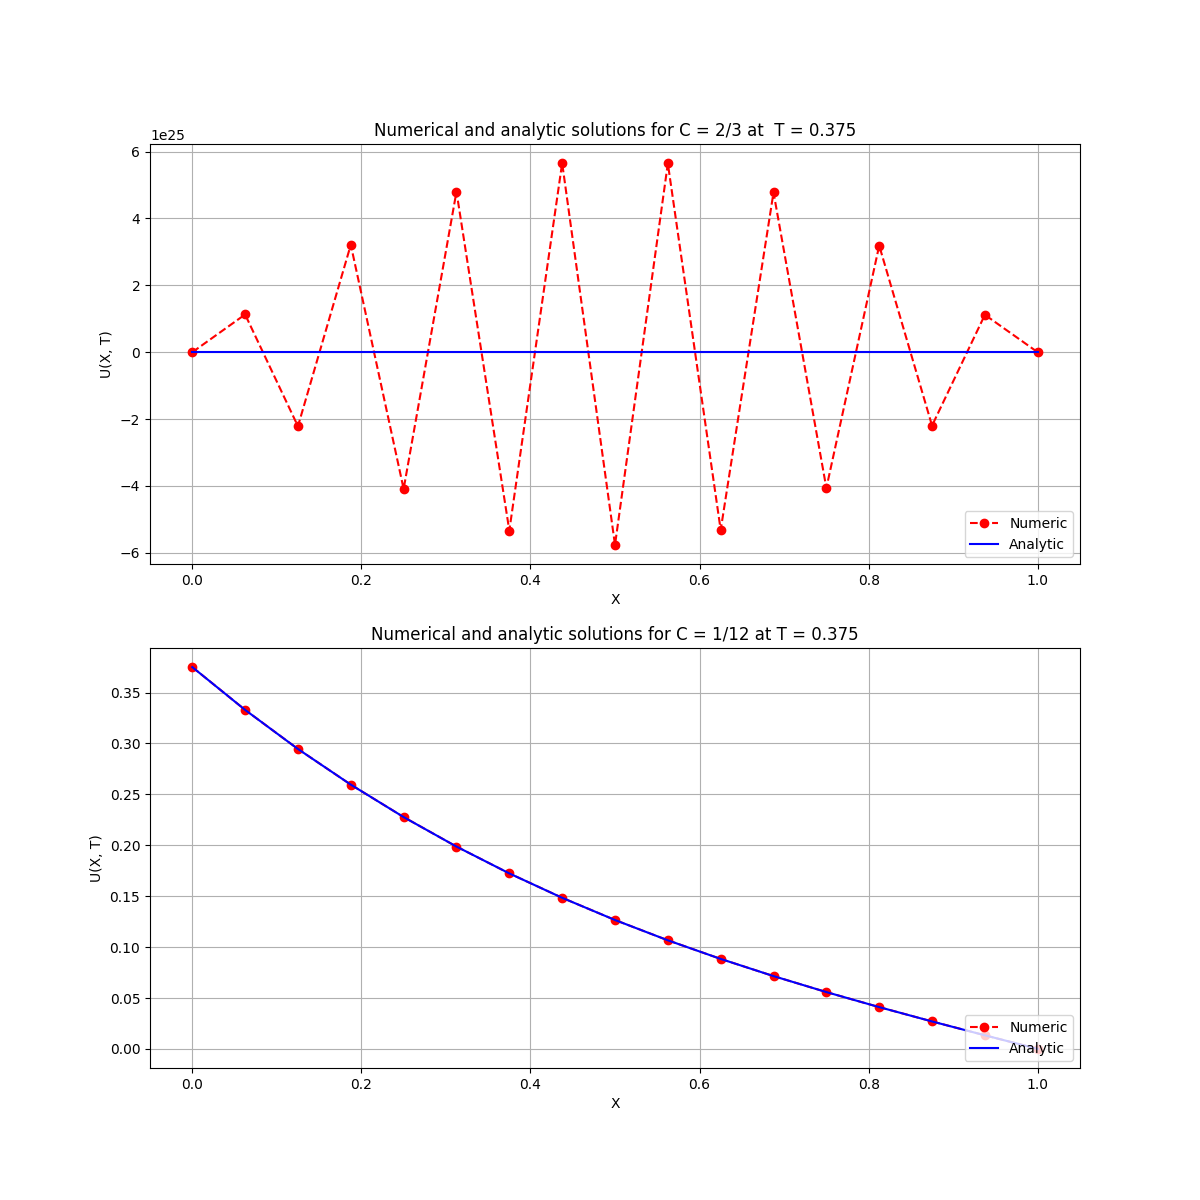
\includegraphics[width=1.0\linewidth]{images/heat_instable.png}
    \caption{Instability for \(C = \frac{2}{3}\), stability for \(C = \frac{1}{12}.\)}
    \label{fig:enter-label}
\end{figure}

Further analysis of changing \(C\) seems to indicate that the scheme is stable when \(C \leq \frac{1}{2\kappa}\) and unstable otherwise (\(\kappa = 1\) in our heat equation). This is in fact a result from Von Neumann stability analysis. One major drawback of the FTCS scheme is when \(\kappa\) is large, the stable step sizes can be too small to be practical. As an aside, using the FTCS scheme for hyperbolic (as opposed to parabolic) equations results in instability for any choice of \(\Delta T\).

To determine accuracy, we shall study the behaviour of the error between the numeric solution and the analytic solution. Recall that our choice of number of terms to sum ensure that the calculation error for the analytic solution is smaller in magnitude than the precision error. We have
\[ \pder[U]{T}(X, T = O(\Delta T) = \frac{U(X, T + \Delta T) - U(X,T)}{\Delta T} \]
and
\[ \spder[U]{X}(X, T) + O((\delta T)^2) = \frac{U(X + \Delta X, T) - 2U(X, T) + U(X - \Delta X, T)}{(\Delta X)^2}, \]
yielding the error 
\(E_n^m = O(\Delta T) + O((\Delta X)^2) \approx A(\Delta X)^2 + B(\Delta T), \)
for some constants \(A, B\) depending on \(\Delta X\), \(\Delta T\) which is first order accurate in time, since for sufficiently small \(\Delta T\), \(\Delta X\) is negligible. 

From the tables, the error seems to grow as \(T\) increases and from the graphs, the error is maximised at \(X = 0.5\). To approximate the coefficients \(A\) and \(B\), let us take \(T = 0.375\) and \(X = 0.5\) and vary \(N\) and \(C\) in such a way to keep one of \(\Delta T\) or \(\Delta X\) fixed.

\begin{verbatim}[Output]
    Fixed DT
    N       C           DX          DT              Error
    4       1/128       1/4         1/2048      3.0778e-04
    8       4/128       1/8         1/2048      6.2525e-05
    16      16/128      1/16        1/2048      4.7540e-06
    32      64/128      1/32        1/2048      -9.4769e-06

    Fixed DX
    32      1/2         1/32        1/(1*2048)  -9.4769e-06
    32      1/4         1/32        1/(2*2048)  -2.3681e-06
    32      1/8         1/32        1/(4*2048)  1.1850e-06
    32      1/16        1/32        1/(8*2048)  2.9624e-06
\end{verbatim}

For the first table, halving \(\Delta X\) appears to quarter the error so behaves quadratically aside from the last row, where \(C = \frac{1}{2}\) is on the boundary between instability and stability. It would be ideal to take \(\Delta X\) smaller, but this shrinks \(\Delta T\) quadratically, and runs into overflow errors due to lack of memory. For the second table, note that whilst we have not taken \(N\) large enough so that \((\Delta X)^2\) is negligible, we can still infer that the difference between the errors which depend only on \(\Delta T\) behave linearly with respect to \(\Delta T\). This gives \(A \approx M \cdot 10^{-3}\) for some \(M \in (0,10)\) and \(B \approx 2 \). 

Since we use two loops, the time complexity of our algorithm is given by \(O((\Delta T \Delta X)^{-1}) = O(N^3)\). This is a significant downside, as the amount of computational power required to ensure stability and high 1st-order accuracy grows rapidly.

\section{Numerical Integration in Python}

The SciPy package has a subpackage integrate which contains several functions for computing integrals. For instance, trapz and simp implements the trapezium and Simpson's rule to compute an integral from given fixed samples.

\begin{minted}[autogobble, linenos]{python}
    import numpy as np
    from scipy.integrate import trapz
    
    a = 0
    b = np.pi
    n = 11
    h = (b - a) / (n - 1)
    x = np.linspace(a, b, n)
    f = np.sin(x)
    
    I_trapz = trapz(f,x)
    I_trap = (h/2)*(f[0] + 2 * sum(f[1:n-1]) + f[n-1])
\end{minted}

Also, quad can be used for general purpose integration given a function.

We can also perform Monte-Carlo integration to estimate the area of a geometric figure given a defining function. This involves using any random package from Python, sampling from a distribution and inferring information based upon where the points lie. The following is an example program which estimates \(\pi\), albeit converging very slowly.

\begin{minted}[autogobble, linenos]{python}
    def pi_estimate(N):
        count = 0
        for _ in range(N):
            x = random.random()
            y = random.random()
            if x**2 + y**2 <= 1:
                count += 1
        return 4 * count / N
\end{minted}

\end{document}
